\documentclass{article}
\usepackage{graphicx} % Required for inserting images
\usepackage{hyperref}
\usepackage{float}
\usepackage[style=apa, backend=biber]{biblatex}

\title{ECON 607 Assignment 3}
\author{Andrew Girgis}
\date{September 2023}
\addbibresource{Assign3/assign3cite.bib}

\begin{document}

\maketitle

\newpage

\tableofcontents

\newpage

\listoffigures

\newpage

\doublespacing

\section{Jaccard Similarity score}
\subsection{What is the Jaccard Similarity score?}
The Jaccard Similarity score is the lexical similarity between two articles of text. It measures the size of the intersection of common words between the two texts divided by the size of the union of the two texts. Using this definition we know that if two documents were identical, say for example if you were to put the same document into the Jaccard Similarity score calculator we would get a Jaccard Similarity score of 1 and conversely if we put to completely different articles where there are no words that intersect we would get a Jaccard Similarity score of 0. Therefore the Jaccard score can only range between 0 and 1

\subsection{How to calculate the Jaccard Similarity score?}
As mentioned in the definition about the Jaccard Similarity, It measures the size of the intersection of common words between the two texts divided by the size of the union of the two texts. By this definition we know that the Jaccard Similarity score is the number of words in commmon divided by the total number of words. The formula for the Jaccard Similarity can be seen in Equation~\ref{Jaccard}.

\begin{equation}
Jaccard(A,B) = \frac{|A \cap B|}{|A \cup B|} = \frac{|A \cap B|}{|A| + |B| - |A \cap B|}
\label{Jaccard}
\end{equation}

\subsection{Jaccard Similarity score analysis}
In this case we are computing the Jaccard Similarity score on an article and the comments on the article. We should expect a low Jaccard Similarity score because the comments on the article are written by individuals typically expressing their own thoughts so most of the words used would be their own and not taken straight from the article. The Jaccard Similarity score computed of the article vs article comments is 0.095. This Jaccard score makes sense since we know that the Jaccard score must be low however individuals will definitely refer to words or phrases used in the article when expressing their opinions. Some real examples we see from the comments include "Do you think human remains would be left in the compost is that why you are saying this?" and "We're gonna end up with a lot of over-caffeinated plants.". In the first example we see that the words "human", "compost" and "remains" would be intersecting with the article however in the second example only the word "lot" overlaps with the article showing that there is definitely variance in the number of words that will overlap with the article however it will more likely be a low amount compared to the whole comment.

\section{Semantic Similarity Score}
\subsection{What is the Semantic Similarity score?}
Semantic Similarity uses an algorithm to map words to numerical vectors so that those appearing together frequently are more proximate. The Semantic Similarity score represents a n-dimensional vector space with each word represented in a vector form (\cite{Majumdar_2022}). The Semantic Similarity score scores words based on how similar they are, even if they are not exact matches.(\cite{Thomas_2020}) This is useful if we want words like 'wheels' and 'engines' to relate to 'cars'. In the Jaccard since they are not exact overlapping words the Jaccard score wouldnt capture this similarity however the Semantic Similarity score does.

\subsection{How to calculate the Semantic Similarity score?}
The Semantic Similarity metric measures the cosine of the angle between two n-dimensional vectors projected in a multi-dimensional space(\cite{Majumdar_2022}). The Semantic Similarity score ranges from 0 to 1, where a score closer to 0 shows there is less similarity and a score closer to 1 shows there is more similarity.

\begin{equation}
Semantic(A,B) = cos \theta = \frac{|A \cdot B|}{||A|| \times ||B||} = \frac{\sum_{i=1}^{n} A_i \times B_i}{\sqrt{\sum_{i=1}^{n} A_{i}^2} \times \sqrt{\sum_{i=1}^{n} B_{i}^2}}
\label{Semantic}
\end{equation}

\subsection{Semantic Similarity score analysis}
As we know we are comparing an article to the comments on the article. Since we know that the Semantic Similarity score will compare words that are alike but don't necessary have to overlap exactly we should be expecting a high Semantic Similarity score. This is because the comments on the article would typically be related to the article contents so words that have similar meanings would be picked up in the Semantic Similarity whereas in the Jaccard the only time the words were in the calculation was if they were exact. The Semantic Similarity score computed for article vs article comments is 0.829. This aligns with our estimate that the Semantic Similarity score would be high, if we look at the example comments we looked at during the Jaccard analysis we can see that in the second comment:  "We're gonna end up with a lot of over-caffeinated plants." we only had the word "lot" with the Jaccard line up with the article however here in the semantic analysis the calculation would take into account the word "plant" since the topic is related to decomposition. This is an example of the Semantic Similarity score giving us a more accurate reading on the relevance of the comments than the Jaccard Similarity score did.

\section{Semantic Intensity score}
\subsection{What is the Sentiment Intensity score?}
Sentiment Intensity analysis is a text analysis method that detects polarity (e.g. a positive or negative opinion) within the text, whether a whole document, paragraph, sentence, or clause (\cite{Beri_2020}). The Sentiment Intensity analysis can be done at the word(token), sentence(span), or document(corpus) level. This is important becuase a sentence like "The steak was good, but the seating could have been better" is a sentence(span) that contains two separate polarities however at the word(token) level the words are all positive without the context.

\subsection{How to we compute the Sentiment Intensity score}
To compute the Sentiment Intensity score we use nltk's VADER package. nltk VADER stands for Valence Aware Dictionary for sEntiment Reasoning and it is a model used for text sentiment analysis that is sensitive to both polarity (positive/negative) and intensity (strength) of emotion. The VADER algorithm is one which links the lexical features of words to emotional intensities. Words such as 'happy' 'love' 'good' 'great' are all seen as positive polarities (positive emotions) however VADER is also smart enough to understand 'was not happy' as a negative polarity (negative emotion) statement.

\subsection{Semantic Intenstiy score analysis}
The sentiment Intensity score returns us a dictionary with the sentiment score in the negative, neutral, positive and compound sentiments. The negative sentiment would calculate how many negative words(tokens) and sentences(spans) are. The positive sentiment would calculate how many positive words(tokens) and sentences(spans) are. If a word(token) or sentence(span) is not positive or negative it is considered neutral. The compound score is the summation of all the scores on a scale of -1 to 1 with -1 being highly negative and 1 being highly positive. After reading the article my opinion is that the author, Brendan Kiley, seems to be neutral in stating that the law has been passed with \parencite[]{Kiley_2019} stating the following
\begin{quote}
"The law, which takes effect May 1, 2020, recognizes “natural organic reduction” and alkaline hydrolysis (sometimes called “liquid cremation”) as acceptable means of disposition for human bodies." (para 2)
\end{quote}
and "This paves the way for Recompose, a project to build the first urban “organic reduction” funeral home in the country." \parencite[]{Kiley_2019}. 
However later in the article they include some quotes from outside sources that seem to be for the new law with quotes seen in \parencite[]{Kiley_2019} such as “I think this is great,” said Joshua Slocum, director of the Funeral Consumers Alliance (para, 10) and “'I think this is great' said Joshua Slocum, director of the Funeral Consumers Alliance" \parencite[]{Kiley_2019}. Due to this I expect there to be a high positive compound sentiment analysis score on this article, since a lot of the article is neutral and positive. The output recieved after running the code was: 
\begin{itemize}
    \item neg: 0.068
    \item neu: 0.822
    \item pos: 0.11
    \item compound: 0.9306
\end{itemize}
As expected, we see that there is a low negative sentiment analysis with the number being close to 0, then we can see the neutral is very high and the positive is greater than the negative which sums up to a positive compound score of 0.9306 showing that the article was more on the positive polarity than on the negative polarity.

\section{Article comment's Sentiment Analysis and Visualization}

\subsection{Positive Comment Matrix}

For the comment matrices we created Gephi network visualizations. The visualization for the positive comments matrix can be seen in Appendix~\ref{sec:PositiveVisualization}. For this diagram I scaled the nodes and words so that if the word comes up more frequently the node and word would be larger and vice versa. I also scaled the size of the edges(arrows connecting the nodes) and coloured the edges so that if the words come up together more often the edge would be larger and more red where as if the words dont come up together as much the edge would be smaller and closer to a light orange. From the network visualization seen in Appendix~\ref{sec:PositiveVisualization} we can see the largest nodes are produced from the words;

\begin{itemize}
    \item Cremation
    \item Composting
    \item Want
    \item Like
    \item Earth
    \item Ash
    \item Body
\end{itemize}

The Gephi network visualization also provides us with a visualization of the words that connect the most within the comments which are signified by the dark red arrows/edges. Based on the figure in Appendix~\ref{sec:PositiveVisualization} we can see that some of the most connected words in the comments include: (Use, Composting, cremation) and (Think, Body, Earth). 

\subsection{Positive Comment Matrix Insights}

Based on the results of our Gephi Network visualization there are many insights we can draw from the data about what is commonly being said within the positive comments. Starting with the words that were used the most \emph{Cremation} and \emph{Composting} are among the top and this makes sense since the article is about using human remains for \emph{composting} via natural organic reduction and alkaline hydrolysis (sometimes called “liquid cremation”) where before this bill was passed Washington code had permitted only burial and \emph{cremation} \parencite[]{Kiley_2019}. The next most used words were words that included the positive sentiment in the VADER analysis \emph{want} and \emph{like}, these words being included in the comment is what allows the nltk VADER algorithm to know that it is indeed a positive comment so it makes sense that we can see these words come up a lot in the positive comments. Finally with regards to the frequency of occurrences some other large words we observed was \emph{earth}, \emph{body} and \emph{ash}. Based on these three words being frequently used in the positive comments we can infer that many comments speak to the \emph{body} being given back to the \emph{earth} instead of turned into \emph{ash}. To confirm this I looked at the words that were used together frequently and saw that \emph{think, body} and \emph{earth} were used together a lot which helps us to infer that most of the people who comment with positive sentiment \emph{think} that the \emph{body} should go back to the \emph{earth}. Another important link found in the Gephi network visualization was \emph{use, compost, cremation}. From this major connection we can infer that many of the comments with positive sentiment believe that we should be \emph{using} human \emph{composting} instead of \emph{cremation} because the cremation of dead bodies uses fossil fuels and a high amount of energy whereas human composting is a more natural process and has a much smaller carbon footprint. 
\begin{quote}
    “Human composting … uses much less energy than cremation, which uses fossil gas to create heat of over 1,400 degrees Fahrenheit,” said Katrina Spade, founder and CEO of Recompose, a licensed green funeral home in Seattle. “When human composting transforms the organic material of our bodies, carbon is also sequestered in the soil created. Rather than being released as carbon dioxide gas through exhaust during a cremation, the carbon matter contained in each body returns to the earth.” \parencite{Rogers_2022}
\end{quote}

\subsection{Negative Comment Matrix}
The visualization for the negative comments matrix can be seen in Appendix~\ref{sec:NegativeVisualization}. From the network visualization we can see the largest nodes are produced from the words;
\begin{itemize}
    \item Family
    \item Death
    \item Hospital
    \item Remains
    \item Human
    \item Casket
    \item Time
\end{itemize}

In the visualization we can also see that the words that connect the most in the negative comments matrix are: (Family, Death, Human) and (Family, Casket, Remains)

\subsection{Negative Comment Matrix Insights}

The results that were produced from the negative comments matrix visualization were quite different from the results produced from the positive comments matrix visualization. The first observation I made when creating the visualizations was that the negative comments matrix visualization has many fewer strong connections between words but more medium strength connections between words where as the positive matrix had a more strong connections between words and less medium strength connections. My inference for this difference in the visualizations is that a lot of the positive comments were using the same point to express there happiness for the bill being passed, that point being that the use of human composting is better than cremations and that it is good for the earth for us to give our body's back to it. Whereas with the negative comments since a lot of the points will be more sentimental we see more variance in the points being made in the negative comments. Another point that caught my eye instantly is that Family and Death connects to a large variety of words, in the positive comments matrix network there is almost a 1 to 1 mapping along the whole network however in the negative comment matrix network the words \emph{Family} and \emph{Death} connect to almost the whole network, my inference for this being that the comments that are against human composting are against it because they want to have a proper send off for the \emph{death} of their \emph{family} members through a burial in a \emph{casket} or would like to keep a token of them to remember them through an urn of their ashes. In the negative comments matrix network we can also see the words \emph{Human} and \emph{Remains} were also used a lot, my inference for these words being used frequently in the negative comments is that individuals who wouldn't be okay with the idea of \emph{human} composting most likely put a lot of value on a \emph{human} body, this could relate to the individuals culture or religion. For example in a Catholic funeral it is customary to have a wake for the deceased where they have a viewing and recite the rosary before they are lowered in the casket. In Hong Kong culture it is customary to scatter the ashes of the deceased in a designated garden of remembrance or out at a designated part of sea \parencite[]{Norris_2019}. This can help us see why the connection between the words \emph{Family, Casket}, and \emph{Remains} is so strong in the negative commments matrix visualization, the comments with a negative sentiment score have a strong tie to the emotional weight of a human body and believe it wrong to not have a ritual for the deceased where the deceased is placed in a casket and buried, and considering that this article is written in the United States of America which is a dominantly Christianity country it makes sense that a large number of the negative comments use that to argue their point.

\newpage

\printbibliography

\newpage

\appendix

\section{Appendix 1}
\label{sec:PositiveVisualization}

\begin{figure}[H]
\caption{Screen capture of the Positive Comments Matrix completed in Gephi}
\begin{center}
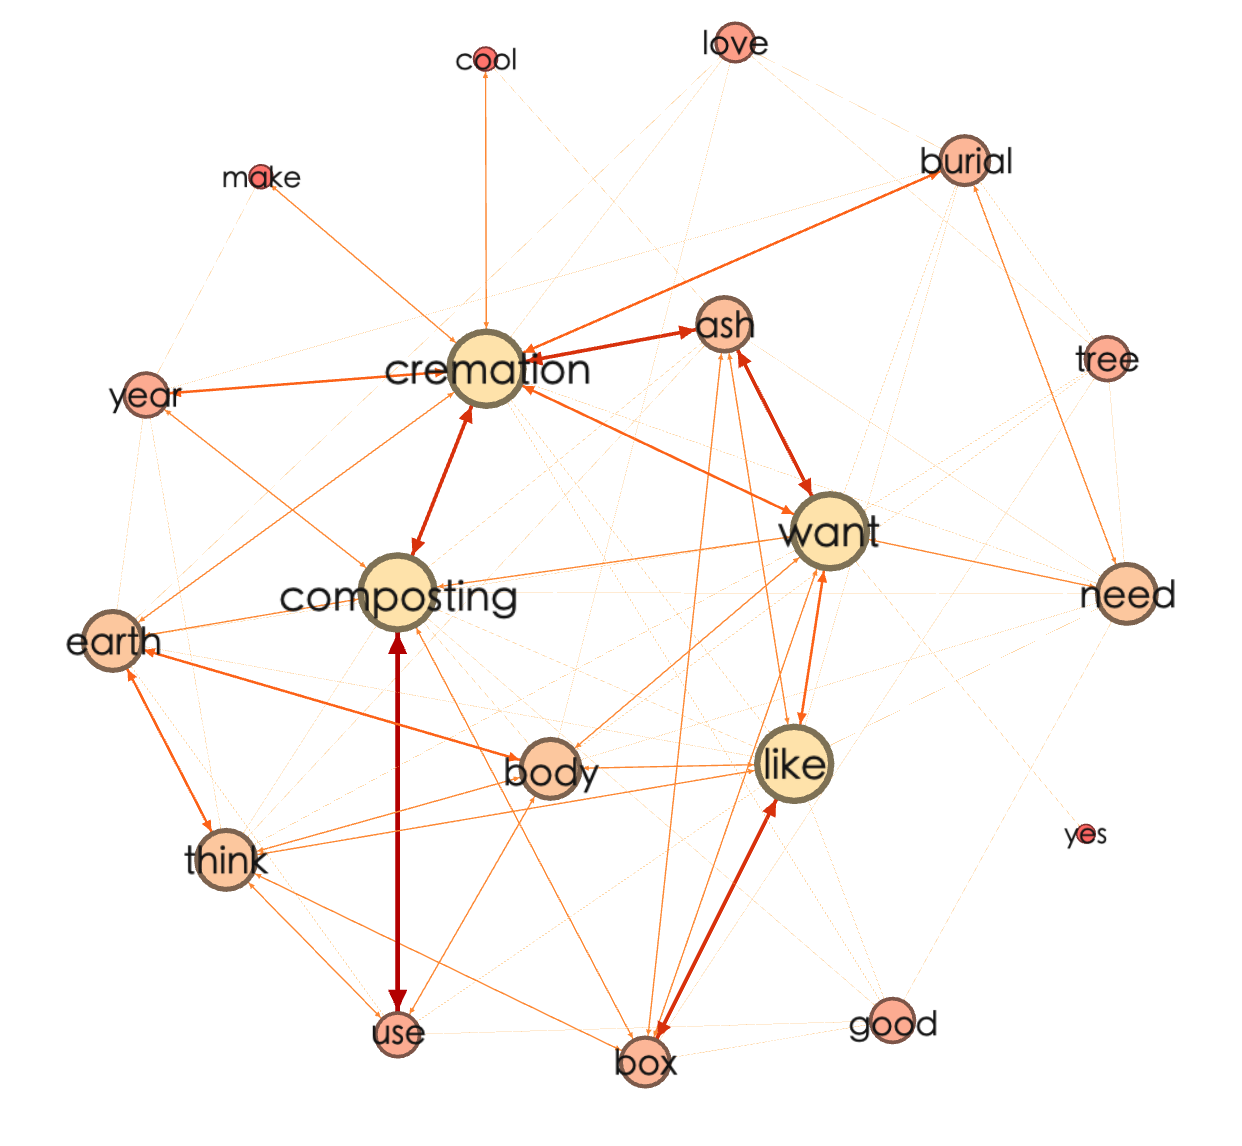
\includegraphics[scale=0.40]{Assign3/PositiveCommentsMatrix.png}
\label{positivecommentsmatrix}
\end{center}
\end{figure}

\newpage

\section{Appendix 2}
\label{sec:NegativeVisualization}

\begin{figure}[H]
\caption{Screen capture of the Negative Comments Matrix completed in Gephi}
\begin{center}
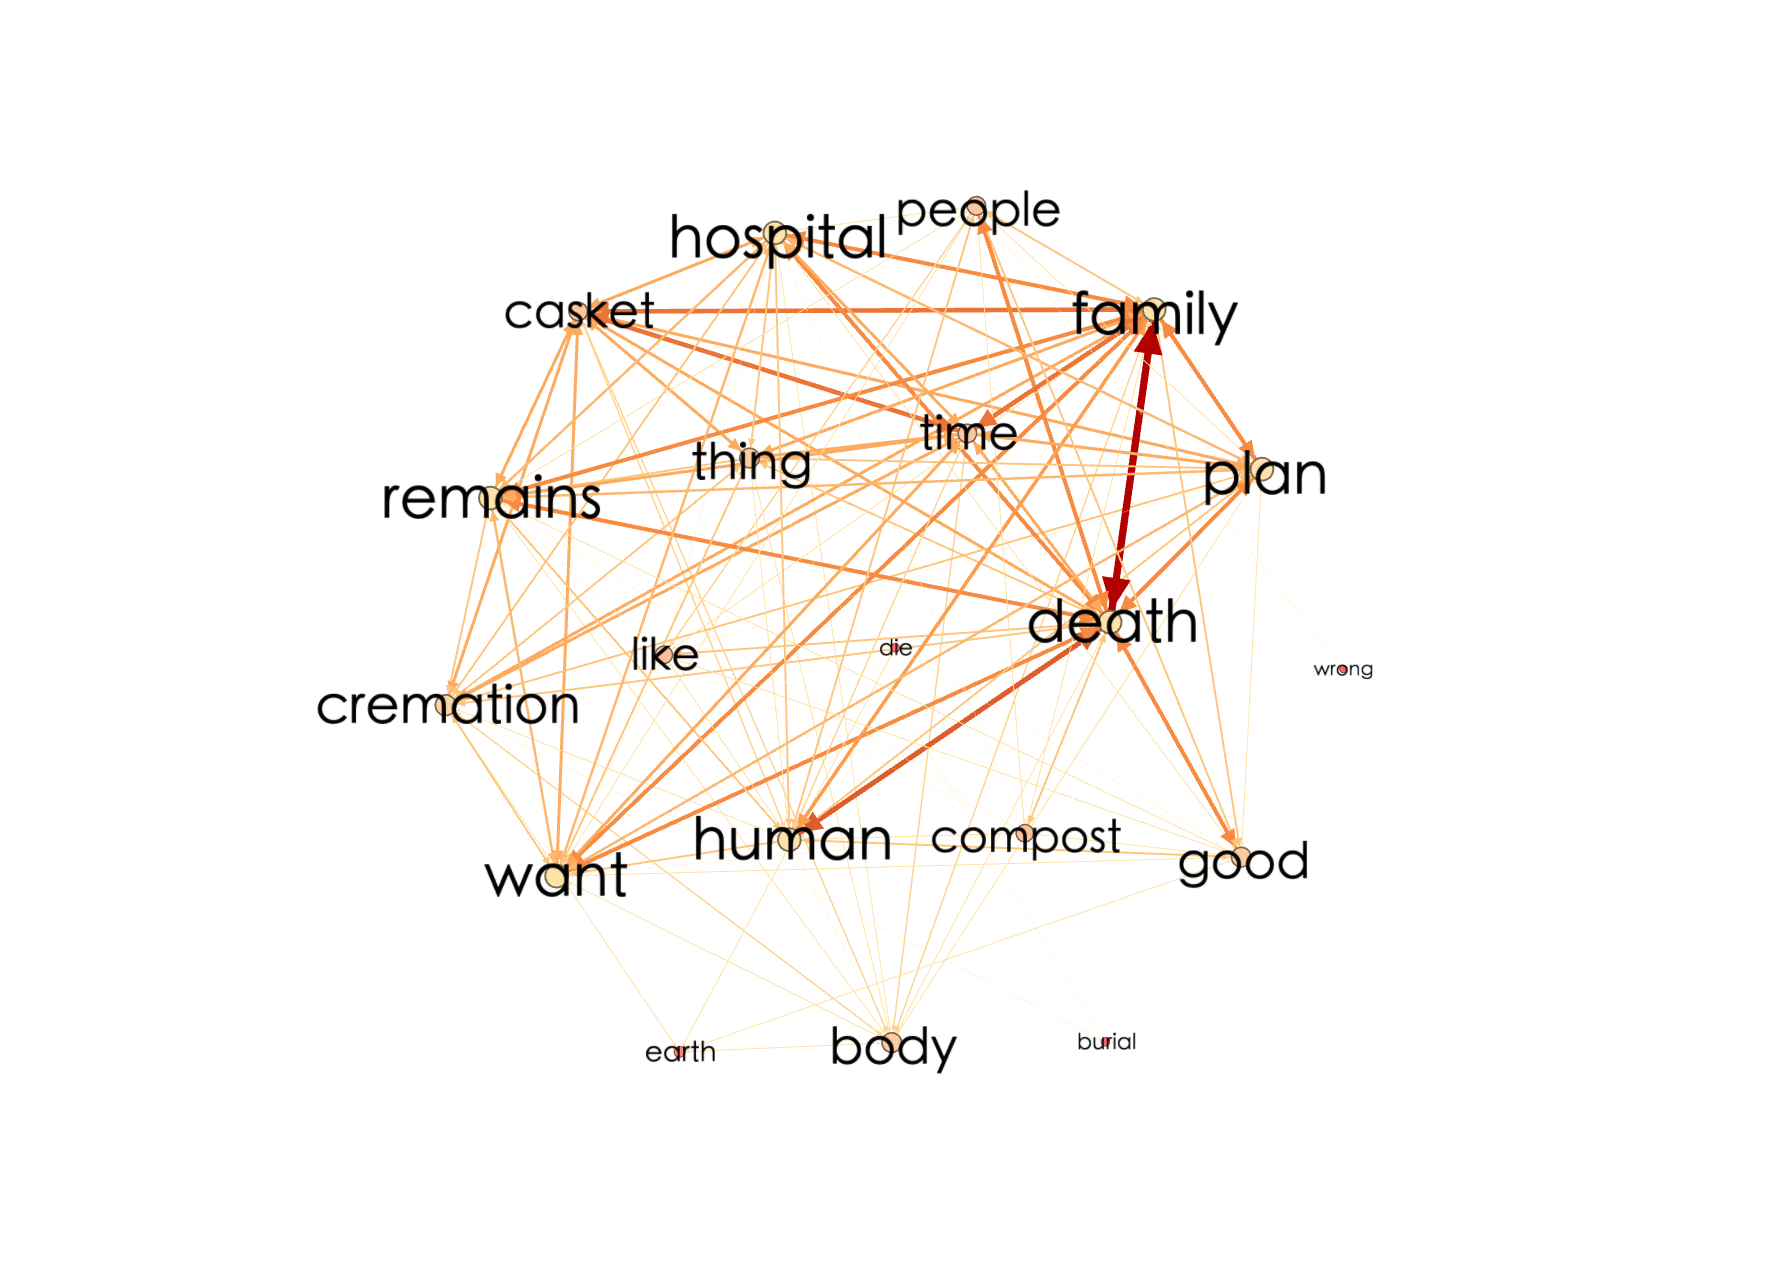
\includegraphics[scale=0.40]{Assign3/NegativeCommentsMatrix.png}
\label{negativecommentsmatrix}
\end{center}
\end{figure}

\newpage

\section{Code}

\begin{verbatim}

# %% [markdown]
# # Import Libraries
# 

# %%
import nltk
from nltk.tokenize import RegexpTokenizer
from nltk.tokenize.treebank import TreebankWordDetokenizer
from nltk.stem import WordNetLemmatizer
from nltk.corpus import stopwords
from nltk.sentiment.vader import SentimentIntensityAnalyzer

import spacy

import pandas as pd

# %% [markdown]
# ## Create a function to calculate the Jaccard Similarity

# %%
def jaccardSimilarity(doc_1, doc_2):
    words_doc1 = set(doc_1.lower().split())
    words_doc2 = set(doc_2.lower().split())
    print(doc_1)
    print(doc_2)
    print(words_doc1)
    print(words_doc2)
    #List the unique words in a document

    intersection = words_doc1.intersection(words_doc2)
    #Find the intersection of words in doc_1 and doc_2

    union = words_doc1.union(words_doc2)
    #Find the union of words in doc_1 and doc_2

    return float(len(intersection)/len(union))
    #Calculate Jaccard Similarity score
    #using length of intersection set divided by length of union set


# %% [markdown]
# ## Create a function to calculate the Semantic Similarity Score

# %%
def semanticSimilarity(doc_1, doc_2):
    spc = spacy.load('en_core_web_lg')
    spacyDoc_1 = spc(doc_1)
    spacyDoc_2 = spc(doc_2)
    return spacyDoc_1.similarity(spacyDoc_2)

# %% [markdown]
# ## Create a function for Sentiment Analysis

# %%
def sentimentAnalysis(doc):
    sia = SentimentIntensityAnalyzer()
    sentiment = sia.polarity_scores(doc)
    return sentiment

# %% [markdown]
# ## Create function for text cleaning

# %%
nltk.download('vader_lexicon')
nltk.download('stopwords')
nltk.download('wordnet')

def cleanText(text):
    tokenizer = RegexpTokenizer(r'\w+')
    allTokens = tokenizer.tokenize(text)
    #Removes puncuation while tokenizing

    tokens = [token for token in allTokens if token not in 
    stopwords.words('English')]
    #Removes the stop words

    tokens = [token.lower() for token in tokens]
    #Convert tokens to lowercase

    lemmatizer = WordNetLemmatizer()
    tokens = [lemmatizer.lemmatize(token) for token in tokens]
    #Lemmatizes the tokens

    text = ''
    for token in tokens:
        text = text + token + ' '
    return text
    # Create a text string from the token list



# %% [markdown]
# ## Create the functions to Load and Clean text

# %%
def loadText(fileName):
    f = open(fileName, 'r', encoding='utf-8')
    text = f.read()
    return text

def loadCleanText(fileName):
    text = loadText(fileName)
    return cleanText(text)

article_2 = loadCleanText('Article2.txt')
commentsArticle_2 = loadCleanText('CommentsA2.txt')
#Loads the data

print("Jaccard: Article 2 vs Article 2 comments", 
jaccardSimilarity(article_2, commentsArticle_2))
#performs the Jaccard similarity calculation

print("Semantic: Article 2 vs Article 2 comments", 
semanticSimilarity(article_2, commentsArticle_2))
#performs the Semantic similarity calculation


# print("Article 2", sentimentAnalysis(article_2))
# comments = loadText('commentsA2.txt').splitlines()
# count = 0
# for comment in comments:
#     count = count + 1
#     comment = cleanText(comment)
#     s = sentimentAnalysis(comment)
#     print(str(count) + ") Comment:", comment + ',', s["compound"])

print("Article 2", sentimentAnalysis(article_2))
comments = loadText('commentsA2.txt').splitlines()
for comment in comments:
    comment = cleanText(comment)
    s = sentimentAnalysis(comment)
    print(comment + ',', s["compound"])

# %% [markdown]
# ## Cooccurance script

# %%
def Preprocessing(corpus):
    # Convert corpus (lines of comments) to an array of comments
    documentText = []
    corpus = corpus.splitlines()
    for row in corpus:
        documentText.append(row)      
    return documentText

# %%
def GenerateMatrix(cleanData, fileName):
    # sklearn countvectorizer
    from sklearn.feature_extraction.text import CountVectorizer
    # Convert a collection of text documents to a matrix of token counts
    cv = CountVectorizer(ngram_range=(1,1), stop_words = 'english', 
    max_features=20)
    # matrix of token counts
    X = cv.fit_transform(cleanData)
    Xc = (X.T * X) # matrix manipulation
    Xc.setdiag(0) # set the diagonals to be zeroes as it's pointless to be 1
    names = cv.get_feature_names_out() # This are the entity names 
    (i.e. keywords)
    df = pd.DataFrame(data = Xc.toarray(), columns = names, index = names)
    #print(df)
    print(fileName)
    df.to_csv(fileName)

# %%
def ProcessCorpus():
    fileName = "positiveComments.csv"
    with open (fileName, "r", encoding='unicode_escape') as myfile:
        data = myfile.read()
        cleanData = Preprocessing(data)
        GenerateMatrix(cleanData, "PositiveCommentsMatrix.csv")

    fileName = "negativeComments.csv"
    with open (fileName, "r", encoding='unicode_escape') as myfile:
        data = myfile.read()
        cleanData = Preprocessing(data)
        GenerateMatrix(cleanData, "NegativeCommentsMatrix.csv")

# %%
ProcessCorpus()

# %%
\end{verbatim}
\end{document}
